\section{1174006 - Kadek Diva Krishna Murti}

\subsection{Soal Teori}
\begin{enumerate}
	\item Jelaskan kenapa kata-kata harus di lakukan vektorisasi. dilengkapi dengan ilustrasi atau gambar.
	\hfill\break
	Kata-kata harus dilakukan vektorisasi agar mudah dalam menentukan kesamaan dari kata-kata tersebut. Misal kata 'Tolong' dengan kata 'Tlg'
	\hfill\break
	\begin{figure}[H]
	\centering
		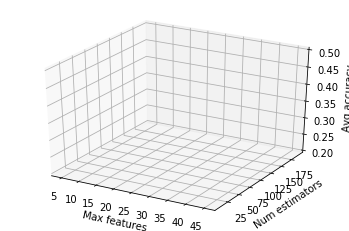
\includegraphics[width=8 cm]{figures/1174006/chapter5/soalteori/v.PNG}
	\end{figure}
	\item Jelaskan mengapa dimensi dari vektor dataset google bisa sampai 300 dilengkapi dengan ilustrasi atau gambar.
	\hfill\break
	
	\hfill\break
	\begin{figure}[H]
	\centering
		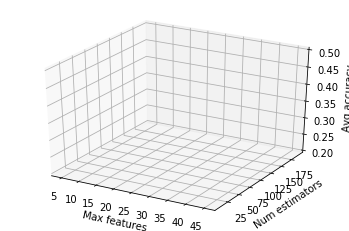
\includegraphics[width=8 cm]{figures/1174006/chapter5/soalteori/v.PNG}
	\end{figure}
	\item Jelaskan konsep vektorisasi untuk kata dilengkapi dengan ilustrasi atau gambar.
	\hfill\break
	
	\hfill\break
	\begin{figure}[H]
	\centering
		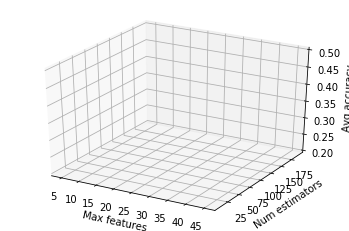
\includegraphics[width=8 cm]{figures/1174006/chapter5/soalteori/v.PNG}
	\end{figure}
	\item Jelaskan konsep vektorisasi untuk dokumen dilengkapi dengan ilustrasi atau gambar.
	\hfill\break
	
	\hfill\break
	\begin{figure}[H]
	\centering
		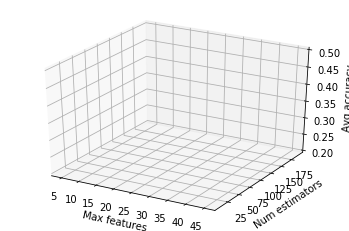
\includegraphics[width=8 cm]{figures/1174006/chapter5/soalteori/v.PNG}
	\end{figure}
	\item Jelaskan apa mean dan standar deviasi dilengkapi dengan ilustrasi atau gambar.
	\hfill\break
	
	\hfill\break
	\begin{figure}[H]
	\centering
		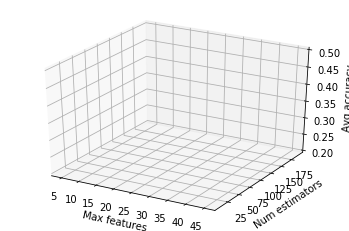
\includegraphics[width=8 cm]{figures/1174006/chapter5/soalteori/v.PNG}
	\end{figure}
	\item Jelaskan apa itu skip-gram dilengkapi dengan ilustrasi atau gambar.
	\hfill\break
	
	\hfill\break
	\begin{figure}[H]
	\centering
		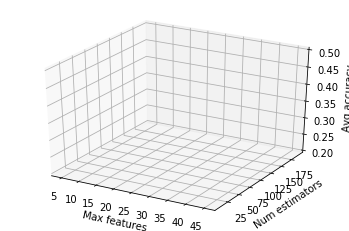
\includegraphics[width=8 cm]{figures/1174006/chapter5/soalteori/v.PNG}
	\end{figure}
\end{enumerate}

\subsection{Soal Praktek}
\begin{enumerate}
	\item Cobalah dataset google, dan jelaskan vektor dari kata love, faith, fall, sick, clear, shine, bag, car, wash, motor, cycle dan cobalah untuk melakukan perbandingan similirati dari masing-masing kata tersebut. Jelaskan arti dari outputan similaritas dan setiap baris kode yang dibuat(harus beda dengan teman sekelas). (Nilai 5 untuk setiap perbandingan, disini ada 5 perbandingan similaritas)
	\hfill\break
	Penjelasan Vektor Per Kata:
	\hfill\break
	Pada kata bag memiliki 300 dimensi vektor sebagai berikut.
	\hfill\break
	\begin{figure}[H]
	\centering
		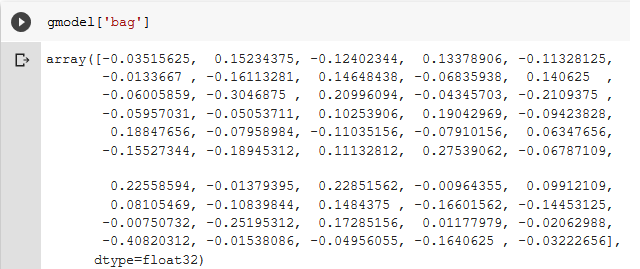
\includegraphics[width=8 cm]{figures/1174006/chapter5/soalpraktek/bag.PNG}
	\end{figure}

	\hfill\break
	Pada kata car memiliki 300 dimensi vektor sebagai berikut.
	\hfill\break
	\begin{figure}[H]
	\centering
		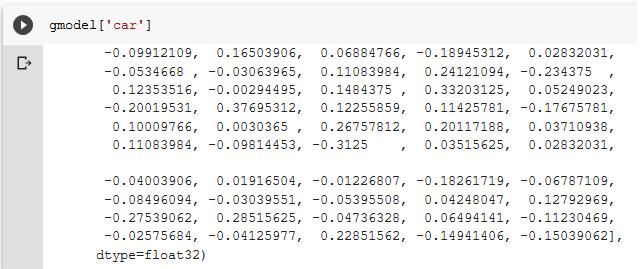
\includegraphics[width=8 cm]{figures/1174006/chapter5/soalpraktek/car.PNG}
	\end{figure}

	\hfill\break
	Pada kata clear memiliki 300 dimensi vektor sebagai berikut.
	\hfill\break
	\begin{figure}[H]
	\centering
		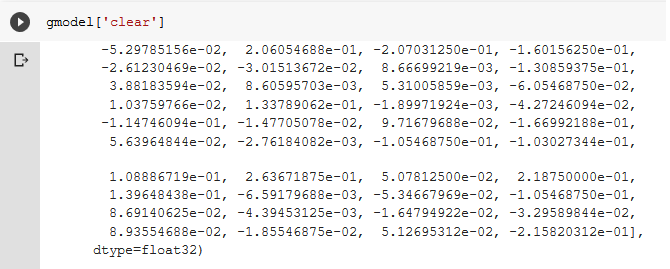
\includegraphics[width=8 cm]{figures/1174006/chapter5/soalpraktek/clear.PNG}
	\end{figure}

	\hfill\break
	Pada kata cycle memiliki 300 dimensi vektor sebagai berikut.
	\hfill\break
	\begin{figure}[H]
	\centering
		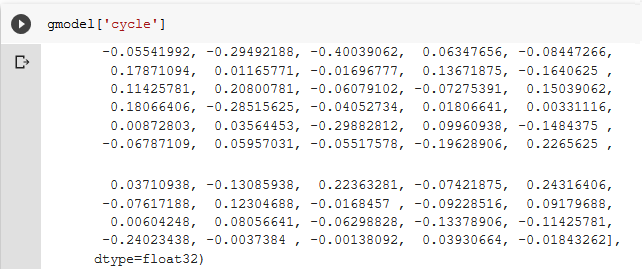
\includegraphics[width=8 cm]{figures/1174006/chapter5/soalpraktek/cycle.PNG}
	\end{figure}

	\hfill\break
	Pada kata faith memiliki 300 dimensi vektor sebagai berikut.
	\hfill\break
	\begin{figure}[H]
	\centering
		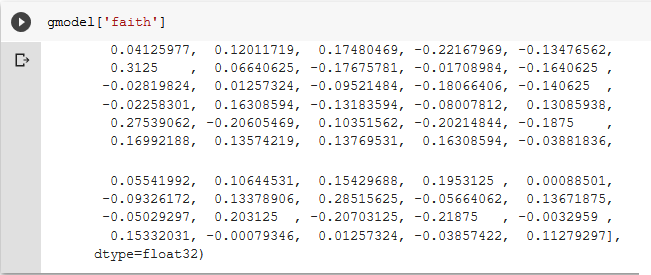
\includegraphics[width=8 cm]{figures/1174006/chapter5/soalpraktek/faith.PNG}
	\end{figure}

	\hfill\break
	Pada kata fall memiliki 300 dimensi vektor sebagai berikut.
	\hfill\break
	\begin{figure}[H]
	\centering
		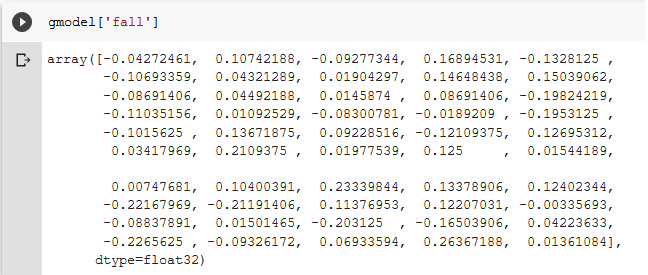
\includegraphics[width=8 cm]{figures/1174006/chapter5/soalpraktek/fall.PNG}
	\end{figure}

	\hfill\break
	Pada kata love memiliki 300 dimensi vektor sebagai berikut.
	\hfill\break
	\begin{figure}[H]
	\centering
		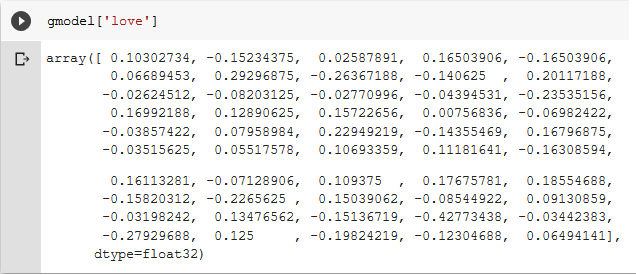
\includegraphics[width=8 cm]{figures/1174006/chapter5/soalpraktek/love.PNG}
	\end{figure}

	\hfill\break
	Pada kata motor memiliki 300 dimensi vektor sebagai berikut.
	\hfill\break
	\begin{figure}[H]
	\centering
		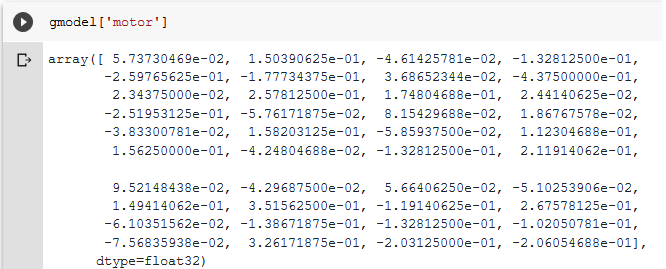
\includegraphics[width=8 cm]{figures/1174006/chapter5/soalpraktek/motor.PNG}
	\end{figure}

	\hfill\break
	Pada kata shine memiliki 300 dimensi vektor sebagai berikut.
	\hfill\break
	\begin{figure}[H]
	\centering
		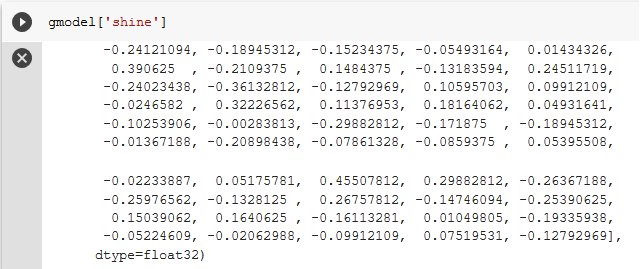
\includegraphics[width=8 cm]{figures/1174006/chapter5/soalpraktek/shine.PNG}
	\end{figure}

	\hfill\break
	Pada kata sick memiliki 300 dimensi vektor sebagai berikut.
	\hfill\break
	\begin{figure}[H]
	\centering
		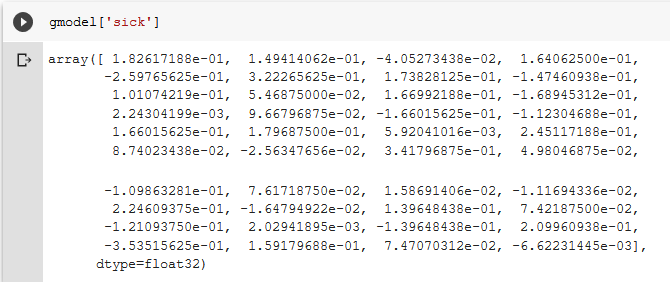
\includegraphics[width=8 cm]{figures/1174006/chapter5/soalpraktek/sick.PNG}
	\end{figure}

	\hfill\break
	Pada kata wash memiliki 300 dimensi vektor sebagai berikut.
	\hfill\break
	\begin{figure}[H]
	\centering
		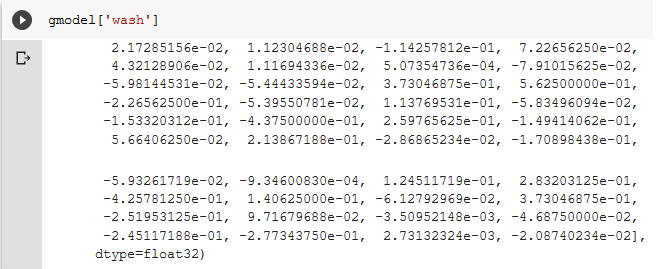
\includegraphics[width=8 cm]{figures/1174006/chapter5/soalpraktek/wash.PNG}
	\end{figure}

	\hfill\break
	Perbandingan Vektor:
	\hfill\break
	Untuk mendapatkan perbandingan similaritas dari dua kata bisa mennggunakan kode berikut.
	\lstinputlisting[firstline=3, lastline=3]{src/1174006/chapter5/praktek.py}
	Disini kita menggunakan method similarity() untuk melakukan perbandingan similarity. Dimana kedua parameternya adalah dua kata yang akan dibandingkan similaritasnya. Hasilnya yaitu berupa angka desimal, dimana semakin mendekati angka 1.0 similaritasnya tinggi begitu juga sebaliknya.
	\hfill\break
	Berikut adalah perbandingan similaritas dari beberapa kata.
	\hfill\break
	\begin{figure}[H]
	\centering
		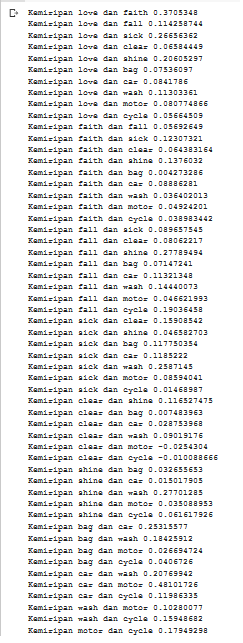
\includegraphics[width=8 cm]{figures/1174006/chapter5/soalpraktek/similarity.PNG}
	\end{figure}

	\item Jelaskan dengan kata dan ilustrasi fungsi dari extract words dan PermuteSentences (harus beda dengan teman sekelas)
	\hfill\break
	Extract Words berfungsi untuk menormalisasi kalimat seperti membuatnya menjadi huruf kecil semua dan menghapus tag HTML, tanda baca dan spasi berulang. Lalu kalimat tersebut dipecah menjadi beberapa kata dan ditampung dalam list. Misal : 'Diva itu Ganteng <b>banget</b>' lalu di extract menjadi ['diva', 'itu', 'ganteng', 'banget']
	\hfill\break
	Permute Sentences berfungsi untuk mengacak atau mengatur ulang kembali urutan dari list kata-kata yang ada. Misal: ['aku', 'adalah', 'kamu'] lalu di permute menjadi ['kamu', 'adalah', 'aku']

	\item Jelaskan fungsi dari librari gensim TaggedDocument dan Doc2Vec disertai praktek pemakaiannya. Tunjukkan keluarannya dari komputer sendiri dan artikan maksud setiap luaran yang didapatkan.
	\hfill\break
	TaggedDocument memiliki fungsi untuk mengklasifikasikan kata berdasarkan tag dari dokumennya. Berikut ini adalah contoh penggunaan TaggedDocument dimana kata-kata yang ada diklasifikasikan sesuai dengan tag dokumennya.
	\hfill\break
	\begin{figure}[H]
	\centering
		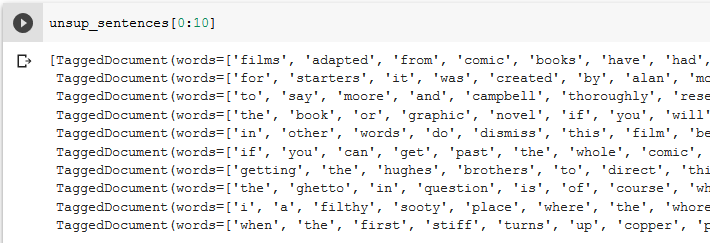
\includegraphics[width=8 cm]{figures/1174006/chapter5/soalpraktek/tagged2.PNG}
	\end{figure}
	\hfill\break
	Doc2Vec memiliki fungsi untuk  training mengkelompokkan kata berdasar kemiripan atribut yang ada. Bisa dibilang Doc2Vec digunakan untuk unsupervised training. Berikut ini adalah contoh penggunaan Doc2Vec dimana kata-kata yang ada dikelompokkan.
	\hfill\break
	\begin{figure}[H]
	\centering
		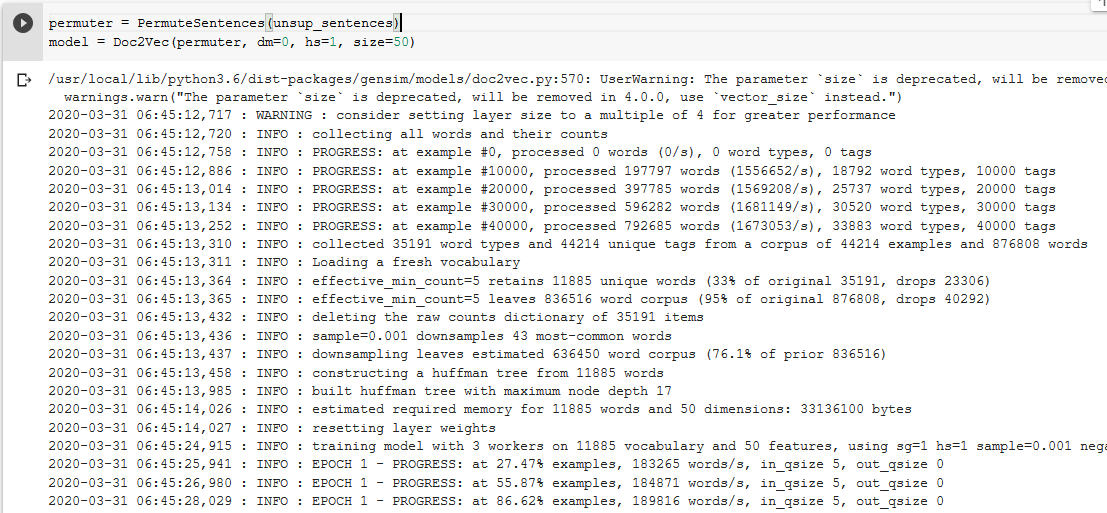
\includegraphics[width=8 cm]{figures/1174006/chapter5/soalpraktek/doc4vec2.PNG}
	\end{figure}

	\item Jelaskan dengan kata dan praktek cara menambahkan data training dari file yang dimasukkan kepada variabel dalam rangka melatih model doc2vec. Tunjukkan keluarannya dari komputer sendiri dan artikan maksud setiap luaran yang didapatkan.
	\hfill\break
	Pertama kita import dulu library yang dibutuhkan.
	\lstinputlisting[firstline=5, lastline=10]{src/1174006/chapter5/praktek.py}
	\hfill\break
	Lalu, buat metode extract\_words()
	\lstinputlisting[firstline=12, lastline=19]{src/1174006/chapter5/praktek.py}
	\hfill\break
	Kemudian panggil dokumen yang ingin di training, lalu dibuat listnya.
	\lstinputlisting[firstline=21, lastline=28]{src/1174006/chapter5/praktek.py}
	\hfill\break
	\begin{figure}[H]
	\centering
		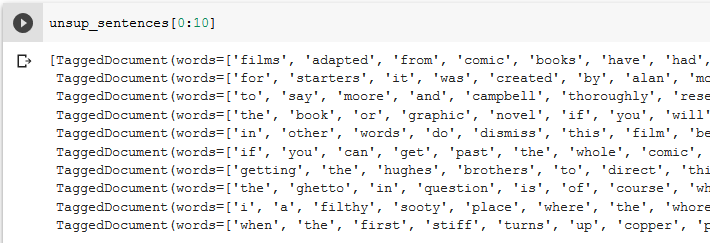
\includegraphics[width=8 cm]{figures/1174006/chapter5/soalpraktek/tagged2.PNG}
	\end{figure}
	\hfill\break
	Setelah itu, buat class PermuteSentences
	\lstinputlisting[firstline=30, lastline=39]{src/1174006/chapter5/praktek.py}
	\hfill\break
	Lalu training dengan Doc2Vec
	\lstinputlisting[firstline=41, lastline=42]{src/1174006/chapter5/praktek.py}
	\hfill\break
	\begin{figure}[H]
	\centering
		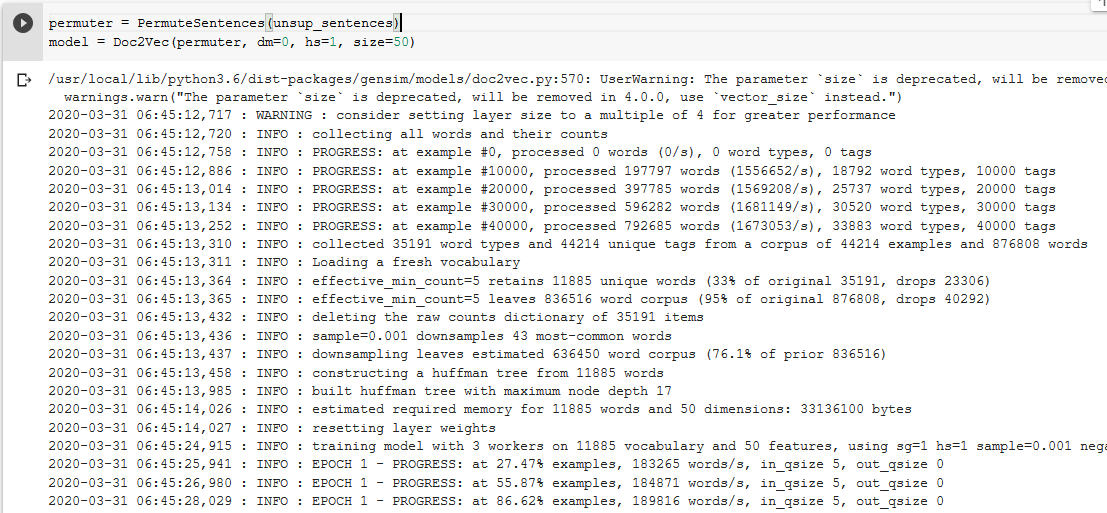
\includegraphics[width=8 cm]{figures/1174006/chapter5/soalpraktek/doc4vec2.PNG}
	\end{figure}

	\item Jelaskan dengan kata dan praktek kenapa harus dilakukan pengocokan dan pembersihan data. Tunjukkan keluarannya dari komputer sendiri dan artikan maksud setiap luaran yang didapatkan.
	\hfill\break
	Pengocokan data dimaksudkan agar datanya lebih bervariasi.
	\lstinputlisting[firstline=30, lastline=39]{src/1174006/chapter5/praktek.py}
	Pembersihan data dimaksudkan agar data yang dipakai untuk training nanti lebih mudah dikenali mesin.
	\lstinputlisting[firstline=12, lastline=19]{src/1174006/chapter5/praktek.py}
	
	\item Jelaskan dengan kata dan praktek kenapa model harus di save dan kenapa temporari training harus dihapus.Tunjukkan keluarannya dari komputer sendiri dan artikan maksud setiap luaran yang didapatkan.
	\hfill\break
	Model harus disimpan agar model tersebut bisa kembali dipakai.
	\lstinputlisting[firstline=45, lastline=45]{src/1174006/chapter5/praktek.py}
	\hfill\break
	Temporari Training harus dihapus agar memori kita tidak penuh untuk keperluan lainnya.
	\lstinputlisting[firstline=47, lastline=47]{src/1174006/chapter5/praktek.py}
	\hfill\break
	\begin{figure}[H]
	\centering
		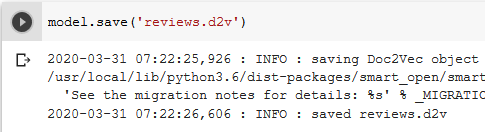
\includegraphics[width=8 cm]{figures/1174006/chapter5/soalpraktek/save.PNG}
	\end{figure}
	\item Jalankan dengan kta dan praktek maksud dari infer code. Tunjukkan keluarannya dari komputer sendiri dan artikan maksud setiap luaran yang didapatkan.
	\hfill\break
	Infer Code dimaksudkan untuk menyimpulkan sebuah dokumen menjadi sebuah vektor.
	\lstinputlisting[firstline=49, lastline=49]{src/1174006/chapter5/praktek.py}
	\hfill\break
	\begin{figure}[H]
	\centering
		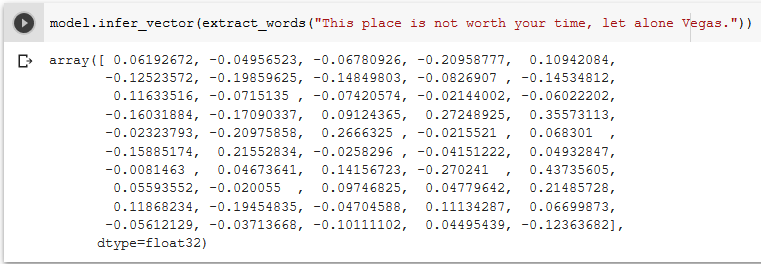
\includegraphics[width=8 cm]{figures/1174006/chapter5/soalpraktek/infen.PNG}
	\end{figure}

	\item Jelaskan dengan praktek dan kata maksud dari cosine similarity. Tunjukkan keluarannya dari komputer sendiri dan artikan maksud setiap luaran yang didapatkan.
	\hfill\break
	Cosine Similarity dimaksudkan untuk memperkirakan seberapa mirip maksud dari kalimat tersebut.
	\lstinputlisting[firstline=51, lastline=54]{src/1174006/chapter5/praktek.py}
	\hfill\break
	\begin{figure}[H]
	\centering
		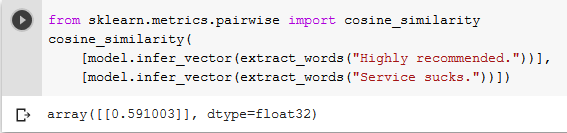
\includegraphics[width=8 cm]{figures/1174006/chapter5/soalpraktek/consine.PNG}
	\end{figure}

	\item Jelaskan dengan praktek score dari cross validation masing-masing metode. Tunjukkan keluarannya dari komputer sendiri dan artikan maksud setiap luaran yang didapatkan.
	
	Pertama kita ambil data dari file dokumen.
	\lstinputlisting[firstline=56, lastline=66]{src/1174006/chapter5/praktek.py}
	\hfill\break
	Lalu bersihkan datanya.
	\lstinputlisting[firstline=68, lastline=70]{src/1174006/chapter5/praktek.py}
	\hfill\break
	Kemudian kita akan menggunakan metode KNN dan Random Forest
	\lstinputlisting[firstline=72, lastline=78]{src/1174006/chapter5/praktek.py}
	Hitung score penggunaan metode Random Forest
	\lstinputlisting[firstline=80, lastline=81]{src/1174006/chapter5/praktek.py}
	\begin{figure}[H]
		\centering
			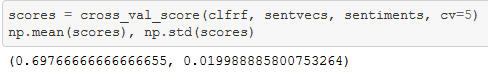
\includegraphics[width=8 cm]{figures/1174006/chapter5/soalpraktek/rf.PNG}
		\end{figure}
	\hfill\break
	Hitung score penggunaan metode KNN
	\lstinputlisting[firstline=83, lastline=84]{src/1174006/chapter5/praktek.py}
	\hfill\break
	\begin{figure}[H]
	\centering
		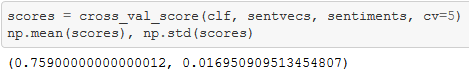
\includegraphics[width=8 cm]{figures/1174006/chapter5/soalpraktek/knn.PNG}
	\end{figure}
\end{enumerate}

\subsection{Penanganan Error}
\begin{enumerate}
	\item Skrinsut error.
	\begin{itemize}
		\item Name Error
		\hfill\break
		\begin{figure}[H]
			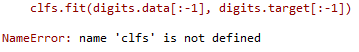
\includegraphics[width=8 cm]{figures/1174006/chapter1/error/err3.PNG}
			\centering
			\caption{Name Error.}
		\end{figure}
		\item Import Error
		\hfill\break
		\begin{figure}[H]
			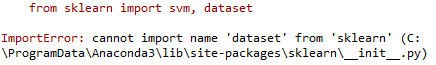
\includegraphics[width=8 cm]{figures/1174006/chapter1/error/err1.PNG}
			\centering
			\caption{Import Error.}
		\end{figure}
		\item Value Error
		\hfill\break
		\begin{figure}[H]
			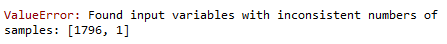
\includegraphics[width=8 cm]{figures/1174006/chapter1/error/err2.PNG}
			\centering
			\caption{Value Error.}
		\end{figure}
		\item Syntax Error
		\hfill\break
		\begin{figure}[H]
			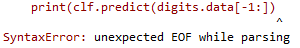
\includegraphics[width=8 cm]{figures/1174006/chapter1/error/err4.PNG}
			\centering
			\caption{Syntax Error.}
		\end{figure}
	\end{itemize}
	\item Tuliskan kode eror dan jenis errornya.
	\begin{itemize}
		\item Name Error
		\hfill\break
		Name Error adalah exception yang terjadi saat syntax melakukan eksekusi terhadap local name atau global name yang tidak terdefinisi.
		\item Import Error
		\hfill\break
		Import Error adalah exception yang terjadi saat syntax melakukan import terhadap library yang tidak terdefinisi.
		\item Value Error
		\hfill\break
		Value Error adalah exception yang terjadi saat syntax memiliki nilai yang tidak valid.
		\item Syntax Error
		\hfill\break
		Syntax Error adalah exception yang terjadi saat ada kesalahan dalam mengetikkan syntax.
	\end{itemize}
	\item Solusi pemecahan masalah error tersebut.
	\begin{itemize}
		\item Name Error
		\hfill\break
		Solusinya adalah memastikan variabel atau function yang dipanggil ada atau tidak salah ketik.
		\item Import Error
		\hfill\break
		Solusinya adalah memastikan library yang dipanggil ada atau tidak salah ketik.
		\item Value Error
		\hfill\break
		Solusinya adalah memastikan nilai yang diinputkan valid.
		\item Syntax Error
		\hfill\break
		Solusinya adalah memastikan syntax yang diketik tidak salah ketik.
	\end{itemize}
\end{enumerate}

\subsection{Bukti Tidak Plagiat}
\begin{figure}[H]
	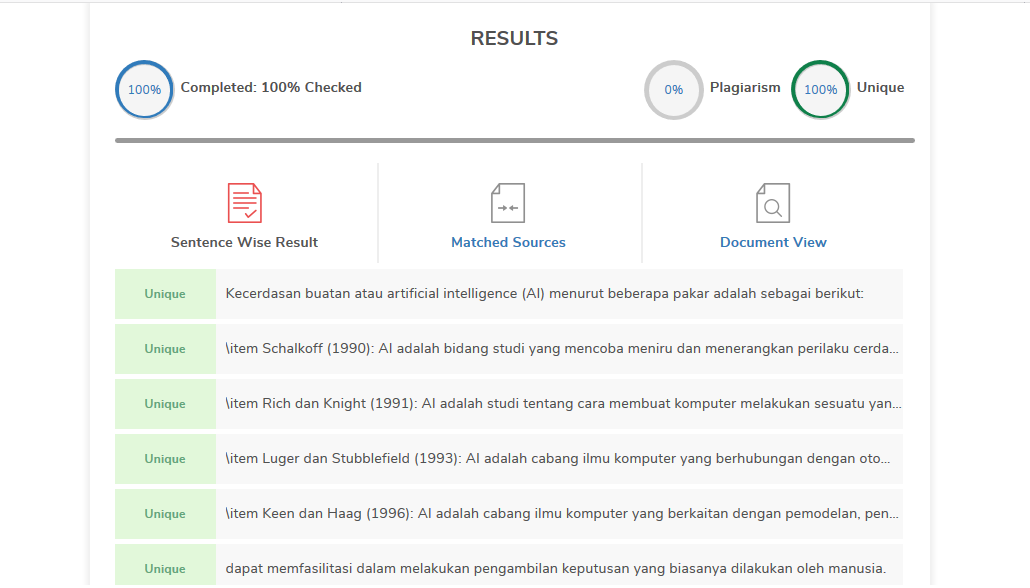
\includegraphics[width=8 cm]{figures/1174006/chapter1/plagiat.png}
	\centering
	\caption{Bukti Tidak Plagiat.}
\end{figure}